\section{Simple\-Modem Class Reference}
\label{classSimpleModem}\index{SimpleModem@{SimpleModem}}
{\tt \#include $<$simplemodem.h$>$}

Inheritance diagram for Simple\-Modem::\begin{figure}[H]
\begin{center}
\leavevmode
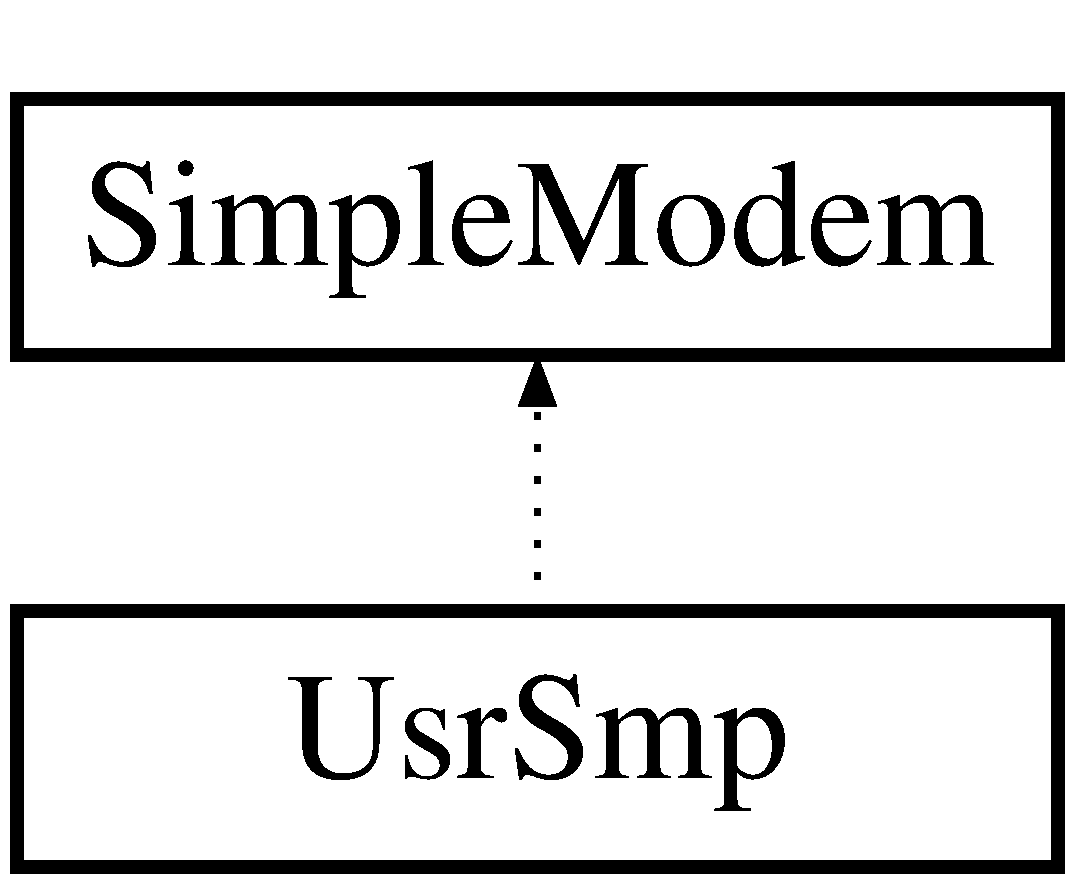
\includegraphics[height=2cm]{classSimpleModem}
\end{center}
\end{figure}
\subsection*{Public Member Functions}
\begin{CompactItemize}
\item 
{\bf Simple\-Modem} (QString interface=\char`\"{}/dev/tty\-S0\char`\"{}, QString baud=\char`\"{}19200\char`\"{})
\begin{CompactList}\small\item\em C'tor. \item\end{CompactList}\item 
{\bf $\sim$Simple\-Modem} ()\label{classSimpleModem_a1}

\begin{CompactList}\small\item\em D'tor. \item\end{CompactList}\item 
QString {\bf Send\-Command} (QString command)
\begin{CompactList}\small\item\em This function sends a command to the modem. \item\end{CompactList}\item 
void {\bf Read\-Memory\-To\-File} (FILE $\ast$fd)
\begin{CompactList}\small\item\em This function reads from the modem and write it to the specified file. \item\end{CompactList}\end{CompactItemize}


\subsection{Detailed Description}
This class implements all necessery function to communicate on a high-level basis with the modem. 



\subsection{Constructor \& Destructor Documentation}
\index{SimpleModem@{Simple\-Modem}!SimpleModem@{SimpleModem}}
\index{SimpleModem@{SimpleModem}!SimpleModem@{Simple\-Modem}}
\subsubsection{\setlength{\rightskip}{0pt plus 5cm}Simple\-Modem::Simple\-Modem (QString {\em interface} = {\tt \char`\"{}/dev/ttyS0\char`\"{}}, QString {\em baud} = {\tt \char`\"{}19200\char`\"{}})}\label{classSimpleModem_a0}


C'tor. 

Mainly for tty init 

\subsection{Member Function Documentation}
\index{SimpleModem@{Simple\-Modem}!ReadMemoryToFile@{ReadMemoryToFile}}
\index{ReadMemoryToFile@{ReadMemoryToFile}!SimpleModem@{Simple\-Modem}}
\subsubsection{\setlength{\rightskip}{0pt plus 5cm}void Simple\-Modem::Read\-Memory\-To\-File (FILE $\ast$ {\em fd})}\label{classSimpleModem_a3}


This function reads from the modem and write it to the specified file. 

Partly (C) T. Uhlmann from usrmodem.cpp \index{SimpleModem@{Simple\-Modem}!SendCommand@{SendCommand}}
\index{SendCommand@{SendCommand}!SimpleModem@{Simple\-Modem}}
\subsubsection{\setlength{\rightskip}{0pt plus 5cm}QString Simple\-Modem::Send\-Command (QString {\em command})}\label{classSimpleModem_a2}


This function sends a command to the modem. 

Call this function to transmit a command to the modem. As result the response of the modem is returned. The function automatically adds a  at the end of the command. 

The documentation for this class was generated from the following files:\begin{CompactItemize}
\item 
simplemodem.h\item 
simplemodem.cpp\end{CompactItemize}
